\documentclass[final_report.tex]{subfiles}

\begin{document}

\section{Initial language comparison}
Before any implementation or specific design considerations were undertaken, an evaluation of the performance of C, Java and the Java Native Interface (JNI) was carried out. Although data from existing articles and websites could be used for Java and C, there was no existing direct comparisons between them and the JNI, therefore custom tests were carried out.

The JNI is inherently \todo{article on this} seen as a bottleneck of an application (even after its vast update in Java 7). \todo{reasons why JNI is slow}

As this application would be forced to use the JNI, numeric values of its performance was helpful to evaluate the bridge in speed required to be overcome.

\subsection{Benchmarking Algorithm}
As discussed previously \todo{ref this}, there are always advantages and disadvantages of any algorithm used for benchmarking. In order to minimise the disadvantages, an algorithm was used which tried to mimic the procedures which would be used in the real application, just without the complications. Algorithm \ref{alg:lang} shows that the program basically creates 100,000 packets individually and populates their fields with random data, which is then processed and return in the 'result' field. This simulates retrieving low-level packet data, interpreting and acting upon the data, and then setting data within the raw packet.

\begin{algorithm}[H]
	\caption{Language Benchmark Algorithm}
	\label{alg:lang}
	\begin{algorithmic}[1]
		\Function{Main}{}
			\For{i = 1 to 100000}
				\State $\textit{p} \gets \textit{Initialise Packet}$
				\State \Call{PopPacket}{p}
				\State \Call{ProPacket}{p}
			\EndFor
		\EndFunction
		\newline
		\Function{PopPacket}{Packet p} \Comment{Set data in a packet}
			\State $\textit{p.a} \gets \textit{randomInt()}$
			\State $\textit{p.b} \gets \textit{randomInt()}$
			\State $\textit{p.c} \gets \textit{randomInt()}$
			\State $\textit{p.d} \gets \textit{randomInt()}$
			\State $\textit{p.e} \gets \textit{randomInt()}$
		\EndFunction
		\newline
		\Function{ProPacket}{Packet p} \Comment{Process a packet}
			\State $\textit{res} \gets \textit{p.a * p.b * p.c * p.d * p.e}$
			\State $\textit{p.result} \gets \textit{res}$
		\EndFunction
	\end{algorithmic}
\end{algorithm}

For the JNI version, the same algorithm was used, however, the \textit{PopPacket} method was carried out on the native side to simulate retrieving raw packet data. The \textit{ProPacket} method was executed on the Java side with the result been passed back to the native side to be entered back into the packet structure.

Timing within the algorithm for all variations was carried out between each iteration. This firstly eliminated any initial start-up time associated with the application which is common with the JVM. Secondly, any calls for time stamps to the system would be miminised as 100,000 iterations would occur in-between them.

\subsection{Results}
Each language had the algorithm run 1,000 times in order to minimise any variations due to external factors. Figures \todo{ref this} show that C was considerably quicker than Java, while Java using the JNI was extremely slow. \todo{expand on this}

\subsection{Further Investigation}
Due to the very poor performance of the JNI compared to other languages, further investigations were carried out to find more specific results surrounding the JNI.
\todo{Is this relevant}

\section{Design Considerations}
\subsection{Data Sharing}
The proposed application will be sharing data between the DPDK code written in C (low level) and the Java (medium level) side used for the highly abstracted part of the application. This requires a large amount of data, most noticeably packets, to be transferred between 'sides' in a small amount of time.
\todo[inline]{Diagram of packets from NIC using c through 'technique' and then processing packets in java and then back}
A few techniques for this are available with Java and C, all with different performances and ease-of-use.

\subsubsection{Objects and JNI - using heap and lots of jni calls}
By far the simplest technique available is using the Java Native Interface (JNI) in order to interact with native code and then retrieve the required via this. This can be done 2 ways, either by creating the object and passing it as a parameter to the native methods or creating an object on the native side via the Java environment parameter. Both ways require the population of the fields to be done on the native side. From then on, any data manipulation and processing could be done on the Java side. Unfortunately, this does require all data to be taken from the object and placed back into the structs before packets can be forwarded. Obviously this results in a lot of unneeded data copying, while the actual JNI calls can significantly reduce the speed of the application as shown in \todo{ref this}.

\subsubsection{ByteBuffers - Non-heap and heap memory}
\todo{bytebuffer uses unsafe but does bound checking}
\todo{cant use bytebuffers directly with DPDK as dont use hugepages}
ByteBuffers are a Java class which allow for memory to be allocated on the Java heap (non direct) or outside of the JVM (direct). Non direct ByteBuffer's are simply a wrapper for a byte array on the heap and are generally used as they allow easier access to bytes, as well as other primitive data types.

Direct ByteBuffers allocate memory outside of the JVM in native memory. This firstly means that the only limit on the size of ByteBuffers is memory itself. Furthermore, the Java garbage collector doesn't have access to this memory. Direct ByteBuffers have increased performance since the JVM isn't slowed down by the garbage collector and intrinsic native methods can be called on the memory for faster data access.

\subsubsection{Java Unsafe - non-heap}
The Java Unsafe class is actually only used internally by Java for its memory management. It generally shouldn't be used within Java since it makes a safe programming language like Java an unsafe language (hence the name) since memory access exceptions can be thrown. It can be used for a number of things such as:

\paragraph*{Object initialisation skipping}
This is where any instance of an object can be created from the class, but no constructors are used meaning that the object created without any of the fields set. This has a number of uses including security check bypassing, creating instances of objects which don't have a public constructor and allowing multiple objects of a singleton class.

\paragraph*{Intentional memory corruption}
This allows the setting of private fields of any object. It is a common way of bypassing security features as private fields to allow access to certain situation can be overwritten to gain access.

\paragraph*{Nullifying unwanted objects}
This has a common use of nullifying passwords after they have been stored as strings. If a password is stored as a string in Java, even setting the field to \textit(null) will only dereference it. The original string will still be in memory after the dereferencing up until it is garbage collected. Even rewriting the field with a new field won't work as strings are immutable in Java. This makes it susceptible to a timing attack to retrieve the password. Using unsafe allows for the actual memory location to be overwritten with random values to prevent this.

\paragraph*{Multiple inheritance}
Java doesn't allow multiple inheritance within its class declaration of casting. However, using Unsafe any object can be cast to any other object without a compiler of run-time error. This obviously only works if data fields are compliant with each other and any method invocations are referenced. 

\paragraph*{Very fast serialization}
The Java \textit{Serializable} abstraction is well known to be slow, which can be a major bottleneck in fast processing applications over a network. Even the \textit{Externalizable} functionality isn't much factor and that requires an class schema to be defined. However, custom serializing can be extremely fast using the Unsafe Class. Basically allocating memory and then putting/getting data from the memory requires little JVM usage and can be done with machine instructions.

Obviously without proper precautions any of these actions can be dangerous and can result in crashing the full JVM. This is why the Unsafe class has a private constructor and calling the static Unsage.getUnsafe() will throw a security exception for untrusted code which is hard to bypass. Fortunately, Unsafe has its own instance called 'theUnsafe' which can be accessed by using Java reflection \todo{ref this}:

\begin{lstlisting}[language=Java, caption={Accessing Java Unsafe}, label=lst:java_unsafe]
Field f = Unsafe.class.getDeclaredField("theUnsafe");
f.setAccessible(true);
Unsafe unsafe = (Unsafe) f.get(null);
\end{lstlisting}

Using Unsafe then allows direct native memory access (off heap) to retrieve data in any of the primitive data formats. Custom objects with a set structure can then be created, accessed and altered using Unsafe which provides a vast increase in performance over traditional objects stored on the heap. This is mainly thanks to the JIT compiler which can use machine code more efficiently. This also removes the need for copying of data between memory locations, structs and objects, therefore meaning it is zero-copy.

\subsubsection{Evaluation}

\subsubsection{JNA?}

\subsubsection{Packing C Structs - in its own section?}
Structs are a way of defining complex data into a grouped set in order to make this data easier to access and reference as shown in Code \ref{lst:c_struct}.

\begin{lstlisting}[language=C, caption={Example C Struct}, label=lst:c_struct]
struct example {
    char *p;
    char c;
    long x;
    char y[50];
    int z;
};
\end{lstlisting}

On modern processors all commercially available C compilers will arrange basic C datatypes in a constrained order to make memory access faster. This has 2 effects on the program. Firstly, all structs will actually have a memory size larger than the combined size of the datatypes in the struct as a result of padding. However, this generally is a benefit to most consumers as this memory alignment results in a faster performance when accessing the data.

\todo[inline]{Explain why it has faster performance}
\todo[inline]{Nested padding in struct?}
\todo[inline]{C struct field always in given order}
\todo[inline]{Inconsistencies with datatype length so using uint32t etc}

Code \ref{lst:c_padded_struct} shows a struct which has compiler inserted padding. Any user wouldn't know the padding was there and wouldn't be able to access the data in the bits of the padding through conventional C dereferencing paradigm (only via pointer arithmetic). This example does assume use on a 64-bit machine with 8 byte alignment, but 32-bit machines or a different compiler may have different alignment rules.

\begin{lstlisting}[language=C, caption={Example C Struct with compiler inserted padding}, label=lst:c_padded_struct]
struct example {
    char *p;       // 8 bytes
    char c;        // 1 byte
    char pad[7];   // 7 byte padding
    short x;       // 2 bytes
    char pad[6];   // 6 byte padding
    char y[50];    // 50 bytes
    int z;         // 4 bytes
};
\end{lstlisting}
\todo[inline]{Mention this is on 64-bit machine and obviously you don't notice padding and order of elements can pay an important part in this}

\todo[inline]{Example making sure compiler doesn't pad}
Since the proposed application in this report requires high throughput of data, the initial thought would be that this optimisation is a benefit to the program. Generally this is the case, but for data which is likely to be shared between the C side and Java side a large amount, data accessing is far quicker \todo{Proof on speed} on the Java side if the struct is packed (no padding). This results in certain structs been forced to be packed when compiled, more noticeably, those used for packet headers.

Packed structures mean there are no gaps between elements, required alignment is set to 1 byte. Also \_\_attribute\_\_((packed)) definition means that compiler will deal with accessing members which may get misaligned due to 1 byte alignment and packing so reading and writing is correct. However, compilers will only deal with this misalignment if structs are accessed via direct access. Using a pointer to a packed struct member (and therefore pointer arithmetic) can result in the wrong value for the dereferenced pointer. This is since certain members may not be aligned to 1 byte. In the below example, unint32 is 4 byte aligned and therefore it is possible for a pointer to it to expect 4 byte alignment therefore resulting in the wrong results.

\begin{lstlisting}[language=C, caption={Example C Struct with compiler inserted padding}, label=lst:c_padded_struct]
#include <stdio.h>
#include <inttypes.h>
#include <arpa/inet.h>

struct packet {
    uint8_t x;
    uint32_t y;
} __attribute__((packed));

int main ()
{
    uint8_t bytes[5] = {1, 0, 0, 0, 2};
    struct packet *p = (struct packet *)bytes;

    // compiler handles misalignment because it knows that
    // "struct packet" is packed
    printf("y=%"PRIX32", ", ntohl(p->y));

    // compiler does not handle misalignment - py does not inherit
    // the packed attribute
    uint32_t *py = &p->y;
    printf("*py=%"PRIX32"\n", ntohl(*py));
    return 0;
}
\end{lstlisting}

On an x86 system (which does not enforce memory access alignment), this will produce

y=2, *py=2

as expected. On the other hand on my ARM Linux board, for example, it produced the seemingly wrong result

y=2, *py=1

However, since a packed struct is much easier to traverse from Java than a padded struct, the decision was made to make certain structs packed within the DPDK framework and then recompile the libraries. This decision could be made since other structs within the DPDK framework were also packed and therefore consideration of this was already made.

Note that if a struct contains another struct, that struct should be packed recursively as-well to ensure the first struct has no padding at all.

Char doesn't have alignment and can start on any address. But 2-byte shorts must start on an even address, 4-byte ints or floats must start on an address divisible by 4, and 8-byte longs or doubles must start on an address divisible by 8. Signed or unsigned makes no difference.

Self-alignment makes access faster because it facilitates generating single-instruction fetches and puts of the typed data. Without alignment constraints, on the other hand, the code might end up having to do two or more accesses spanning machine-word boundaries. Characters are a special case; theyÕre equally expensive from anywhere they live inside a single machine word. ThatÕs why they donÕt have a preferred alignment.

casting to an odd pointer will slow down code and could work. Other architectures will take the word which the pointer points to and therefore the problem occurs above.

\subsubsection{Javolution}


\subsection{Performance testing}
In order to evaluate the most suitable data sharing technique, performance testing on 4 different implementation options for sharing data between Java and native memory were considered. Since the ultimate aim of the implementation is to maximise throughput of packets, the performance test tried to mimic this by processing data on 1 million packets per iteration. This processing involved retrieving data from the native packet struct, loading that data into a Java object, changing the data and then setting the data back into the original struct. Various techniques to do this were used to try and find the best performance possible. All of the techniques made use of a static native struct which acted like a new packet been received. The changed data was then set back into this struct.

\begin{algorithm}[H]
	\caption{Data Sharing Performance Test Algorithm}
	\label{alg:data}
	\begin{algorithmic}[1]
		\Function{Main}{}
			\For{i = 1 to 10}
				\State startTimer
				\State \Call{performTest}{ }
				\State stopTimer
				\State outputTime				
			\EndFor
		\EndFunction
		\newline
		\Function{performTest}{}
			\For{i = 1 to 1000000}
				\State retreiveData
				\State setNewData
				\State saveData
			\EndFor
		\EndFunction
	\end{algorithmic}
\end{algorithm}

Considering there were 4 different data sharing techniques tested, the \textit{retrieveData}, \textit{setNewData} and \textit{saveData} methods were different and are described below:

\paragraph*{Objects}
The object technique involved creating a packet and sending its reference through the JNI to the native code. From there, this packet could be populated with data from a given struct through the Java environment pointer. For each setter method called, the method id of that method must be retrieved for the given class so the combination of that and the packet reference could set the data.

From there, new data is input into the packet from the Java side and passed back through to JNI so the struct can be set with the new data. This is done using getters for the objects' fields via the Java environment pointer.

\paragraph*{ByteBuffer}
The technique involved declaring a direct byte buffer to assign off heap memory of the size of the packet struct. From there, the pointer to this memory location was sent to the native code, where data from the struct was directly copied into the byte buffer, therefore populating the byte buffer with duplicate data. The Java code then pulled the data from this via the byte buffer's inbuilt methods and set the data into a new packet object. From there the packet object could be used whenever desired.

To save the data back into the original struct, the data was copied from the packet object back into the byte buffer in the order of the members of the struct. The data was then pulled from the memory of the byte buffer and set back into the original struct.

\paragraph*{Unsafe}
Using the Unsafe class allows for direct access to members of the struct. To take account for this this technique first allocates off heap memory for the pointer to the struct to be stored. This pointer is put into the memory location natively and accessed via Unsafe methods. From this, data can be accessed directly from the struct and input to a new packet object for later use. New data is then set in the object.

To set the data in the struct, the data is removed from the object and directly put into the struct. This is done using the pointer and the correct byte offsets depending on the previous data type inputted.

\paragraph*{Direct}
Direct accessing relates to not storing the struct members in Java at all. Instead a different type of Packet object is used which just stores pointers to the struct. From there any accessing and setting of data is simply done using the Unsafe class to directly get or set the values within the struct. This different packet object also contains offset information for the struct so the correct values are accessed.

\subsubsection{Expectations}
Of the 4 techniques, it is expected that the object method would be by far the slowest, mainly due to the excessive number of JNI calls used which significantly slows an application down. The Byte Buffer method will most likely be the slowest of the other 2 techniques due to the large number of data copying which goes on. The other 2 techniques (unsafe and direct) will likely be very close in performance, mainly because they both use direct accessing into the struct. The unsafe technique should be slightly slower however due to the setting and getting from the packet object.

\todo{evaluate each technique on ease and number of data copies and results and say why we picked 1 of the others}

\subsubsection{Results}
The graphs below show the results from the different techniques run on different systems. Considering there were 10 iterations of 1 million packets per technique the results show the averages of the times. However, certain times were disregard and seen as anomalies since they were well above the average \todo{stats for this}. These were generally at the start of the new technique and can be either be related to the just in time compiler warming up after switching to a different class or garbage collection on the previous technique.

The graphs show the time in nanoseconds which it tool to process an individual packet. The scale is logarithmic due to the excessive size of the object technique. For easier reading, the numbers at the top of the columns show the times factor for each technique comapared to the fastest. For example, on Figure \todo{ref this} the byte buffer takes 2.74 times the direct technique to process the packet.

\begin{figure}[H]
	\centering
	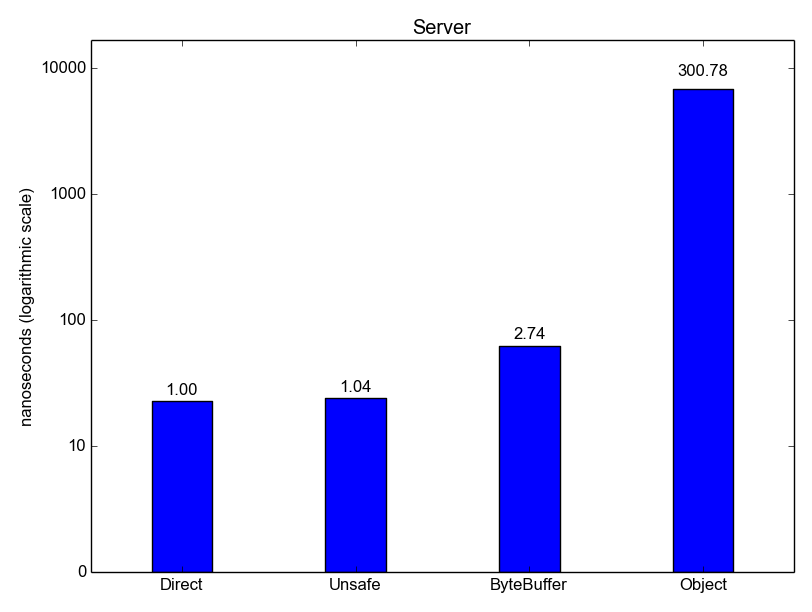
\includegraphics[width=0.8\textwidth]{img/server.png}
	\caption{Server}
	\label{fig:layers}
\end{figure}

\begin{figure}[H]
	\centering
	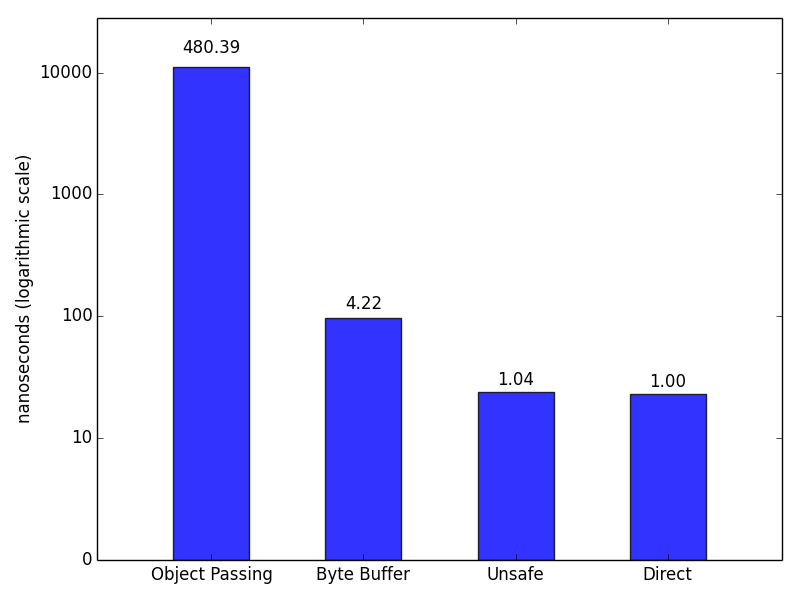
\includegraphics[width=0.8\textwidth]{img/mac.png}
	\caption{Mac}
	\label{fig:layers}
\end{figure}

\begin{figure}[H]
	\centering
	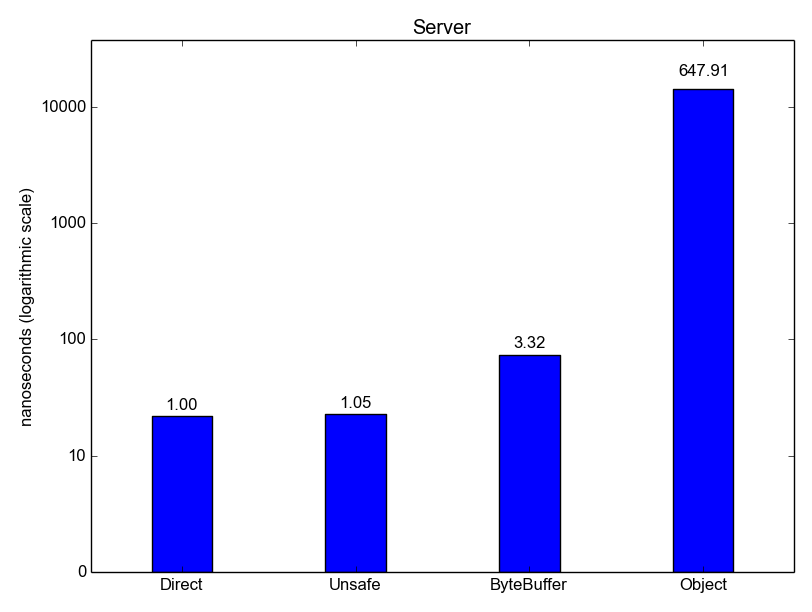
\includegraphics[width=0.8\textwidth]{img/vm.png}
	\caption{VM}
	\label{fig:layers}
\end{figure}

\todo[inline]{should these graphs all be together because they look the same}

\subsubsection{Evaluation}
As the graphs show, the exceptions declared earlier have been met. The object technique should be completely disregard, even though it offers the easiest solution. Due to its abysmal performance, been 300 - 650 times slower than the faster technique, its not going to help with packet throughput.

For similar reasons Byte buffer should be disregarded as well simply because its too slow compared to the other methods. The amount of data copying with this technique is the downfall, although this could have potentially worked if structs could be directly written into the buffers. \todo{cant be done and reference earlier}

The difference between the direct and unsafe methods is minimal on all 3 machines. The direct technique is slightly faster since it doesn't copy the data into the object although Java is surprisingly fast at this as proven by the unsafe results. Furthermore, in general middleware software, there isn't the requirement to access all data fields of the packets generally, therefore storing them all in objects can be seen as needless copying. This is where the direct access technique excels since it only accesses data which it needs to been zero-copy. Direct access was therefore chosen as the technique to use for the implementation which goes into further details about how this was done.

\todo[inline]{extension to remove packet pointer passing and do it directly from struct array - would have to dynamically pack array though - how????}

\todo[inline]{do hardware testing - ie hardware faster than programs (i think) so should aim for throughput and not efficiency}

\subsection{Thread affinity}
Thread.currentThread().getId(); just gets id of thread relative to jvm.

It keeps a process limited to certain a certain core or cores. Process will still be taken out of use and switched back in but without the problem of moving cache between cores.

Normally as a thread gets a time slice (a period in which to use the core), it is granted whichever core [CPU] is determined to be most free by the operating system's scheduler. Yes, this is in contrast to the popular fallacy that the single thread would stay on a single core. This means that the actual thread(s) of an application might get swapped around to non-overclocked cores, and even underclocked cores in some cases. As you can see, changing the affinity and forcing a single-threaded CPU to stay on a single CPU makes a big difference in such scenarios. The scaling up of a core does not happen instantly, not by a long shot in CPU time.

Therefore, for primarily single (or limited) thread applications, it is sometimes best to set the CPU affinity to a specific core, or subset of cores. This will allow the 'Turbo' processor frequency scaling to kick in and be sustained (instead of skipping around to various cores that may not be scaled up, and could even be scaled down).

core thrashing - ust by the name, you know this is a bad thing. You lose performance when a thread is swapped to a different core, due to the CPU cache being 'lost' each time. In general, the *least* switching of cores the better. One would hope the OS would try to avoid this, but it doesn't seem to at all in quick tests under Windows 7. Therefore, it is recommended you manually adjust the CPU affinity of certain applications to achieve better performance.

Another important issue is avoiding placing a load on a HyperThreaded (non-physical) core. These cores offer a small fraction of the performance of a real core. The Windows scheduler is aware of this and will swap to them only if needed. As of mid Jan 2012 the Windows 7 and Windows 2008 R2 schedulers have a hotfix for AMD Bulldozer CPUs that see them as HyperThreaded, cutting them down from 8 physical cores to 4 physical cores, 8 logical cores. This is for two reasons: The AMD Bulldozer platform uses pairs of cores called Bulldozer Modules. Each pair shares some computation units, such as an L2 cache and FPU. To spread out the load and prevent too much load being placed on two cores that have shared computational units, the Windows patch was released, boosting performance in lightly threaded scenarios.

Processor affinity takes advantage of the fact that some remnants of a process that was run on a given processor may remain in that processor's memory state (for example, data in the CPU cache) after another process is run on that CPU. Scheduling that process to execute on the same processor could result in an efficient use of process by reducing performance-degrading situations such as cache misses. A practical example of processor affinity is executing multiple instances of a non-threaded application, such as some graphics-rendering software.

\begin{lstlisting}[language=C, caption={Example of setting thread affinity}, label=lst:c_affinity]
cpu_set_t cpuset;	\\ structure used to manage cpu affinity settings
pthread_t thread = pthread_self();  \\ get own system wide thread id
CPU_ZERO(&cpuset); \\ zero cpuset structure
CPU_SET(5, &cpuset); \\ set cpuset structure use with the 6th core (0-5)
int res = pthread_setaffinity_np(thread, sizeof(cpu_set_t), &cpuset); \\ set affinity of thread
\\ error handling here of res
res = pthread_getaffinity_np(thread, sizeof(cpu_set_t), &cpuset); \\ check affinity of thread
\\ error handling here of res
\end{lstlisting}
\todo{ref this}

In Linux, Java thread uses the native thread(i.e, thread provided by Linux).
This means the JVM creates a new native thread when the Java code creates a new Java thread. So, the Java threads can be organised in any way the native threads can be organised.

A native thread can be bound to a core through the pthread\_setaffinity\_np() function. So, a Java thread can be bound to a core. If Java standard library does not provide a function to do so, then this function need to be provided through JNI.

In Linux, multi-threading is same as parallel threading. Linux kernel distribute threads among processors to balance the cpu load. However the individual threads can be bound with any core as wished. So, in Linux Java multi-threading is same as parallel threading.

\subsection{Endianness}
This describes the order in which bytes of data types are stored in memory relative to pointers. In big-endian systems, the most significant bytes are stored at the pointer with every successive data bytes stored in successive memory locations. Conversely, in little-endian systems, the least significant byte is stored at the pointer. There is no advantage or disadvantage to either endian types, its simply a matter on convention for certain systems. Figure \ref{fig:endian} shows how different endian systems store the value of the hexadecimal value \textit{0x0A0B0C0D}. 

\begin{figure}[H]
	\centering
	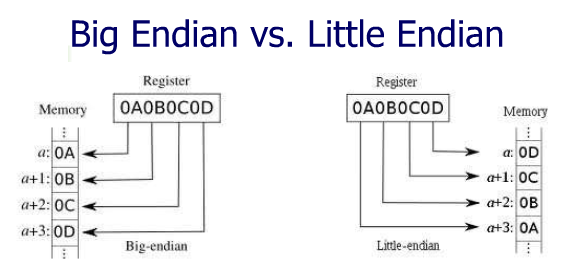
\includegraphics[width=\textwidth]{img/endian.png}
	\caption{Difference between little and big endian}
	\label{fig:endian}
\end{figure}

This becomes a problem when using the Java Native Interface with native code code on Intel architectures since the Java Virtual Machine uses big-endian format while Intel uses little-endian format. Normally the JNI environment would handle this byte ordering conversion but since the JNI has been proven to be too slow \todo{ref this} to meet the requirement, this needs to be handled by the application.

\subsection{Data type conversion}
Between different languages the same data type can be represented by varying lengths in bytes and whether unsigned or signed (in the case of numerical values). It can also be the case that data type lengths in native languages differ depending on the architecture and whether it is 32-bit or 64-bit.

This becomes more of an issue when sharing data between C and Java. Java always uses a signed integer representation with the most significant bit representing whether the number is negative or positive. C uses both signed and unsigned representation depending on the requirements with varying byte length. Again, any conversion between the differences is normally handled via the JNI, but since the implementation aims to bypass the JNI as much as possible, data type conversion will have to be handled.

Lets take the integer representation as an example. In C, and integer can vary between 2, 4 and 8 bytes in length depending on the architecture and compiler. To solve this, standard integer types are used (e.g. uint8\_t \& int32\_t) which guarantee that the representation is at least the length of the type definition stated. In Java, an integer is guaranteed to be 4 bytes long regardless of the system. However, DPDK uses unsigned integers while Java uses signed integers. This requires conversion between the unsigned and signed, but since unsigned has a higher upper bound on the value it can store due to the extra bit (MSB) there can be an overflow error when converting to Java. This requires that Java uses a long (8 byte) representation to hold the C 4 byte unsigned integer.

Conversion from Java to C then could then result in an underflow error if a value which can be represented by a Java long can't be represented by a C integer. This means bound checking is required on the Java side for any number conversions.

\todo{write java code to check and make own exception}
\todo{get a table of this}

\subsection{Protocol undertaking}
just IP (4 and ) supporting udp and tcp (i think), no ARP etc

\subsection{config files}

\end{document}